\section{Concentration Dependent Reaction}
	
	In this section we consider the reaction as a concentration dependent quantity. This is
	
	
	\begin{align}
		J_{x=0} = -D\frac{\partial C}{\partial x}\big|_{x=0} = -R,
	\end{align}
	
	where $R$ is given by the Langmuir absorption model \cite{langmuir}
	
	\begin{align}
		R = \frac{k_fC(0, t)}{1 + K_{eq}C(0, t)},
	\end{align} 
	
	where $k_f$ is a constant proportional to the number of available sites in the solid surface and  and $K_{eq}$ is the equilibrium constant of the reduction of copper reaction at the interface.
	
	If $K_{eq} << k_f$, we can expand this into what is known as the Freundlich formula,
	
	\begin{align}
		R \approx k_f C(0, t),
	\end{align} 
	
	with $k_f = k/K$. For this case, we get the following boundary condition for the flux
	
	\begin{align}
		J_{x=0} = -k_fC(0^+,t),
	\end{align}
	
	which yields a Robin type of boundary condition for our system
	
	\begin{align}
		 \frac{\partial C}{\partial x}\big|_{x=0} -\frac{k_f}{D}C(0^+,t) = 0.
	\end{align}
	
	Thus, we need to solve the following system
	
		
	\begin{align}
		\frac{\partial C}{\partial t} = D \frac{\partial^2 C}{\partial x^2},
		\label{eq:dynamic-system}
	\end{align}
	
	\begin{align}
		C(x = \delta, t) =& C_b,\\
		\frac{\partial C}{\partial x}\big|_{x=0} -\frac{k_f}{D}C(0^+,t) =& 0,\\
		C(x, t=0) =& 0.
		\label{eq:border-conditions-dynamic}
	\end{align}





	\subsection{Steady State}
	
	First, we will solve the steady state solution of this equation,
	
	\begin{align}
		\frac{\partial C_{SS}}{\partial t} = D \frac{\partial^2 C_{SS}}{\partial x^2} = 0,
		\label{eq:steady-state}
	\end{align}
	
	\begin{align}
		C(\delta, t) =& C_b,\\
		\frac{\partial C}{\partial x}\big|_{x=0} -\frac{k_f}{D}C(0^+,t) =& 0.\\
		\label{eq:border-conditions}
	\end{align}
	
	From \ref{eq:steady-state}, we get
	
	\begin{align}
		C_{SS}(x) = A x + B.
	\end{align}


Boundary conditions \ref{eq:border-conditions} yield

\begin{align}
	A\delta + B = C_b,\\
	A-\frac{k_f}{D} B = 0.
\end{align}

From which we get

\begin{align}
	A = \frac{C_b}{1+\frac{k_f\delta}{D}}\frac{k_f}{D},\\
	B = \frac{C_b}{1+\frac{k_f\delta}{D}}.
\end{align}

Therefore,

\begin{align}
	C_{ss} = \frac{C_b}{1+\frac{k_f\delta}{D}} \qty{\frac{k_fx}{D} + 1}.
	\label{eq:steady-state-sol}
\end{align}


\subsection{Dynamic Solution}

Know we consider the complete system \ref{eq:dynamic-system}. To solve this system we define the dimensionless fluctuations with respect to the steady state as

\begin{align}
	\rho(x, t) = \frac{C(x,t) - C_{SS}(x)}{C_b},
\end{align}


which hold the following boundary conditions, which are derived from \ref{eq:border-conditions-dynamic}



\begin{align}
			\rho(\delta, t) =& 0,\\
		\frac{\partial \rho}{\partial x}\big|_{x=0} -\frac{k_f}{D}\rho(0^+,t) =& 0,\\
		\rho(x, t=0) =& -\frac{C_{SS}(x)}{C_b}.
\end{align}


First, we will change variables

\begin{align}
	\xi = \frac{x}{\delta},\\
	\tau = \frac{D t}{\delta^2}.
\end{align}

The dimensionless system is

\begin{align}
		\frac{\partial \rho}{\partial \tau} = \frac{\partial^2 \rho}{\partial \xi^2},
		\label{eq:dynamic-system}
	\end{align}

\begin{align}
			\rho(\xi = 1, \tau) =& 0,\\
		\frac{\partial \rho}{\partial \xi}\big|_{\xi=0} -\frac{k_f\delta}{D}\rho(0^+,\tau) =& 0,\\
		\rho(x, t=0) =& -\frac{C_{SS}(x)}{C_b}.
\end{align}


We use separation of variables. Let

\begin{align}
	\rho(\xi, \tau) =  G(\tau) F(\xi).
\end{align}

In a similar procedure as in section \ref{sec:analytic-diffusion-reaction} we get the following two equations

\begin{align}
	F''(\xi) = -\lambda^2 F(\xi), 
	\label{eq:F-equation}\\
	G'(\tau) = -\lambda^2 G(\tau).
	\label{eq:G-equation}
\end{align}

Note that boundary conditions can be rearrange as


\begin{align}
			F(\xi=1) =& 0,\\
		\qty{\frac{d F(\xi)}{d \xi}\bigg|_{\xi=0} -\frac{k_f\delta}{D}F(0^+)} =& 0.
\end{align}


The solution to equation \ref{eq:G-equation} is

\begin{align}
	G(\tau) = G(0)e^{-\lambda^2 \tau}.
\end{align}

A particular solution to equation \ref{eq:F-equation} is
\begin{align}
	F(\xi) = A_\lambda \cos(\lambda \xi) + B_\lambda \sin(\lambda\xi).
\end{align}

Boundary conditions yield

\begin{align}
	B\lambda - \frac{k_f\delta}{D}A = 0,
	\label{eq:border-eq}\\
	A \cos(\lambda) + B \sin(\lambda) = 0.
\end{align}

From these we obtain that the eigenvalues of the Sturm-Liouville problem $\lambda$ satisfy the following transcendent equation

\begin{align}
	\frac{\tan\lambda}{\lambda} = -\frac{D}{k_f\delta}.
	\label{eq:lambda-equation}
\end{align}

The general solution is then,

\begin{align}
	\rho(\xi,\tau) = \sum_\lambda G(0)e^{-\lambda^2 \tau}\qty{ A_\lambda \cos(\lambda\xi) + B_\lambda \sin(\lambda\xi)}.
\end{align}

From \ref{eq:border-eq} we get

\begin{align}
	\rho(\xi,\tau) = \sum_\lambda A_\lambda e^{-\lambda^2 \tau}\qty{  \cos(\lambda\xi) + \frac{k_f \delta}{D\lambda} \sin(\lambda\xi)},
\end{align}

or equivalently

\begin{align}
	\rho(\xi,\tau) = \sum_\lambda A_\lambda e^{-\lambda^2 \tau}\qty{  \cos(\lambda\xi) - \cot(\lambda)\sin(\lambda\xi)}.
\end{align}

In appendix \ref{apendix:cossin-orthogonality} we show that the functions 

\begin{align}
	P_\lambda(\xi) = \cos(\lambda\xi) - \cot(\lambda)\sin(\lambda\xi),
\end{align}

are orthogonal such that,

\begin{align}
	\left< P_\lambda , P_{\lambda'}\right> &= 0, \\
	\left< P_\lambda , P_{\lambda'}\right> &= -\frac{\qty{\cot\qty{\lambda} -  \lambda \csc^2\qty{\lambda}}}{2\lambda}.
\end{align}

Thus, the Fourier coefficients can be obtained from the initial condition,
 

\begin{align}
	\rho(\xi,\tau = 0) = \sum_\lambda A_\lambda \qty{  \cos(\lambda\xi) - \cot(\lambda)\sin(\lambda\xi)} = -\frac{C_{SS}(\xi)}{C_b}.
\end{align}


Using \label{eq:orthogonality}, 

\begin{align}
\sum_{\lambda'} A_{\lambda'} \delta_{\lambda, \lambda'}\qty{-\frac{\qty{\cot\qty{\lambda} -  \lambda \csc^2\qty{\lambda}}}{2\lambda} }= -\int_0^1 \frac{C_{SS}(\xi)}{C_b}\qty{\cos(\lambda \xi) - \cot(\lambda) \sin(\lambda\xi)}d\xi.
\end{align}




Substituting \ref{eq:steady-state-sol} we get

\begin{align}
A_{\lambda} &= \frac{2\lambda}{\qty{\cot\qty{\lambda} -  \lambda \csc^2\qty{\lambda}}}\int_0^1 \qty{\frac{1+\frac{k_f\delta}{D}\xi}{1+\frac{k_f\delta}{D}}}\qty{\cos(\lambda \xi) - \cot(\lambda) \sin(\lambda\xi)}d\xi,\\
&= \frac{2\lambda}{\qty{\cot\qty{\lambda} -  \lambda \csc^2\qty{\lambda}}}I.
\end{align}

  
The integral $I$ can be computed to yield (using equation \ref{eq:lambda-equation})
\begin{align}
I &= \int_0^1 \qty{\frac{1+\frac{k_f\delta}{D}\xi}{1+\frac{k_f\delta}{D}}}\qty{\cos(\lambda \xi) - \cot(\lambda) \sin(\lambda\xi)}d\xi\\
&= \int_0^1 \qty{\frac{1-\lambda \cot(\lambda)\xi}{1-\lambda \cot(\lambda)}}\qty{\cos(\lambda \xi) - \cot(\lambda) \sin(\lambda\xi)}d\xi,\\
&= \frac{1}{\lambda\sin\qty{\lambda}}.
\end{align}

 we obtain,



\begin{align}
A_{\lambda} = \frac{2\lambda}{\lambda \sin(\lambda)\qty{\cot\qty{\lambda} -  \lambda \csc^2\qty{\lambda}}},
\end{align}

or equivalently
\begin{align}
A_{\lambda} = \frac{2 \sin\qty{\lambda}}{\sin\qty{\lambda}\cos\qty{\lambda}-\lambda}.
\end{align}

Therefore the general solution for this case is

\begin{align}
	\rho(\xi,\tau) = \sum_\lambda  \frac{2\sin(\lambda)e^{-\lambda^2\tau}}{\sin(\lambda)\cos(\lambda)-\lambda}\qty{\cos{(\lambda\xi)} - \cot\qty{\lambda}\sin\qty{\lambda\xi}}.
\end{align}

With 

\begin{align}
	\tan(\lambda) = -\frac{D\lambda}{k_f\delta}.
\end{align}






\begin{figure}[htbp]
\centering
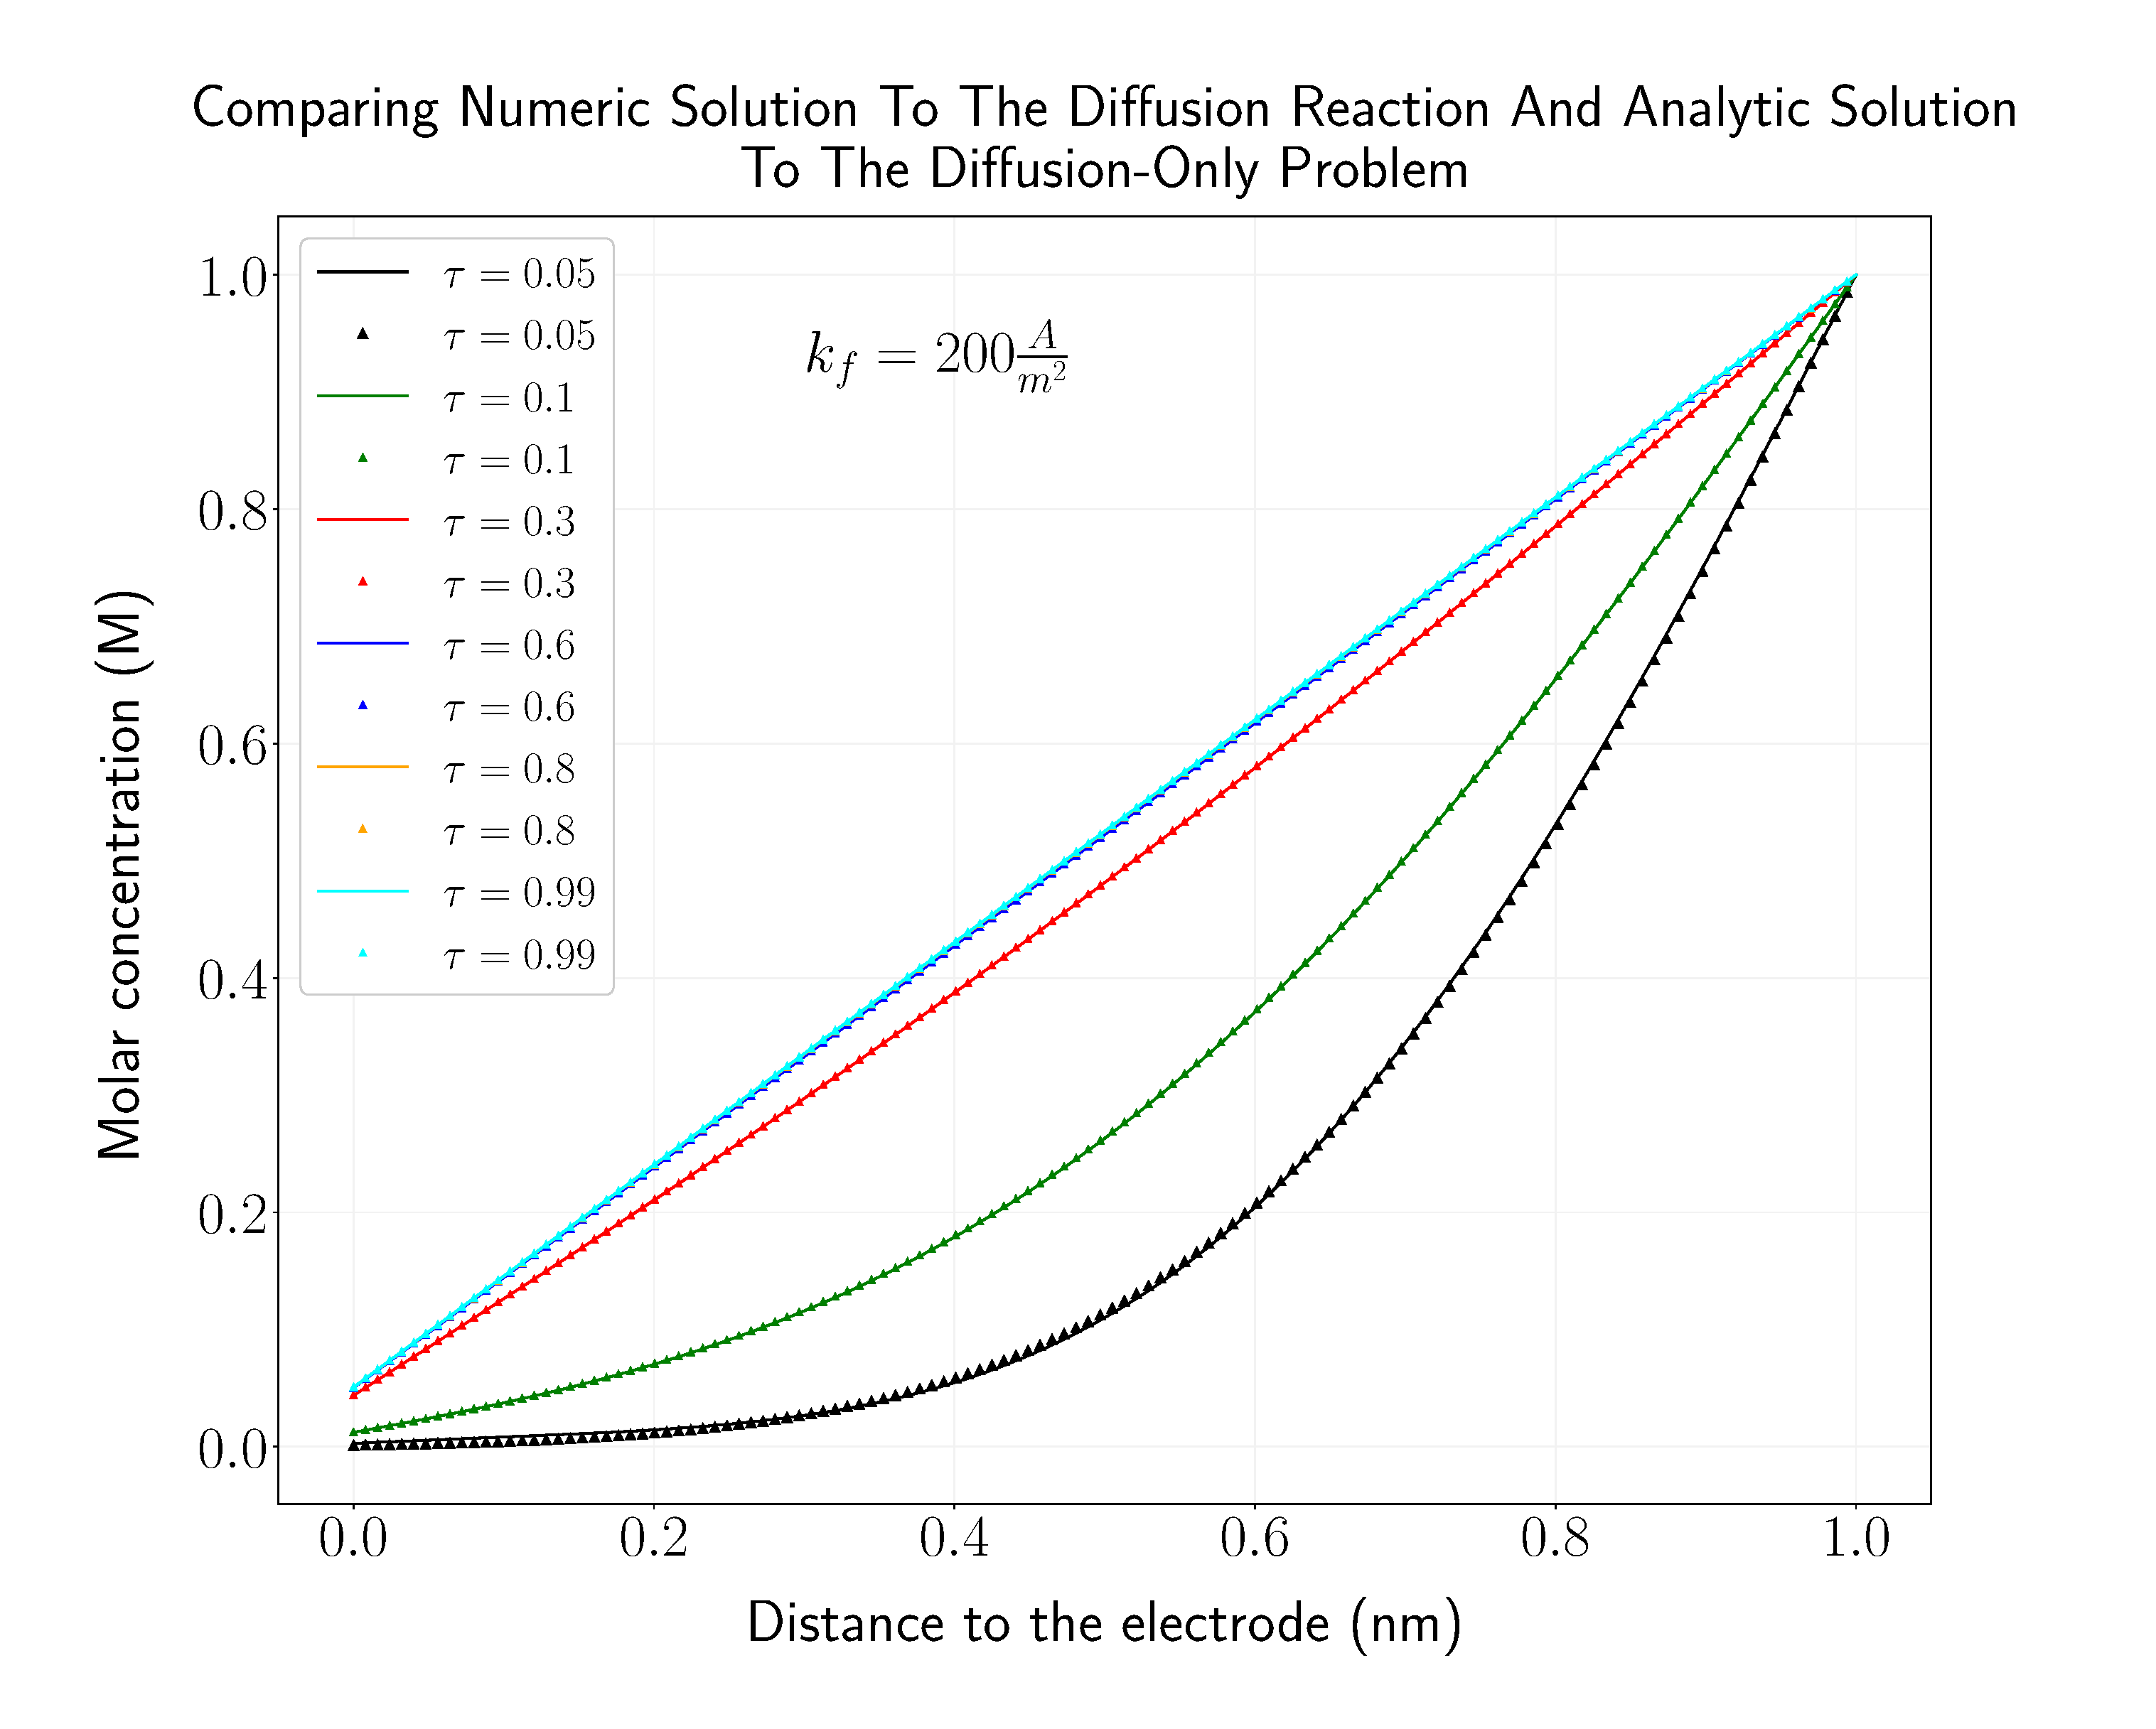
\includegraphics[width=\textwidth]{concentration-diffusion-reaction-robin-comparison}
\caption{In this model, the boundary conditions are physically sensible as the depend on charge carriers to arrive at the interface to produce current. At small $t$ there is no current as copper ions have not reached the surface at $x-0$ and it increases linearly with concentration as time goes on.}
\label{fig:diffusion-reaction-comparison}
\end{figure}
